\documentclass[10pt,english]{beamer}
%\documentclass[english,handout]{beamer} % For handouts
\usetheme[progressbar=frametitle,block=fill]{metropolis} %numbering=none

%%% USEFUL PACKAGES
%\usepackage{showframe} % For debugging positioning
\usepackage{etex} % If too many packages
% Encoding and language
\usepackage[utf8]{inputenc}
\usepackage{babel}
\usepackage{amsmath, amssymb}
\usepackage{natbib}
%\usepackage{booktabs}
%\usepackage{algorithmic}
\usepackage{algorithm}
\usepackage{caption}
%\usepackage{animate} % Animations
\usepackage{bm} % Bold math
\usepackage{bbm}
%\usepackage{url}
%\usepackage{pifont}
%\usepackage{ulem} % Used for strikeouts \sout
%\usepackage{stackengine}
%\usepackage{enumitem}
%\setlist[description]{leftmargin=\parindent,labelindent=\parindent}
%\usepackage{colortbl} % Used for colored rows in tables


%%% GRAPHICS
\usepackage{graphicx}
\graphicspath{{./figs/}}


%%% COLORS
\setbeamercolor{background canvas}{bg=white}
\def\BlankFrame{
	\bgroup
	%\pdfpageheight 29.7cm
	\setbeamercolor{background canvas}{bg=}
	\begin{frame}[plain]
	\end{frame}
	%\makeatletter
	%\pdfpageheight \beamer@paperheight
	%\makeatother
	\egroup}

\usepackage{xcolor}
\definecolor{DarkGreen}{HTML}{00B200}
\definecolor{LightBlue}{HTML}{0090D9}
\definecolor{gold}{rgb}{.812,.710,.231}
% Text markup
%\setbeamercolor{alerted text}{fg=red}
\newcommand{\blue}[1]{\textcolor{blue}{#1}}
\newcommand{\red}[1]{\textcolor{red}{#1}}
\newcommand{\grey}[1]{\textcolor{gray}{#1}}
\newcommand{\orange}[1]{\textcolor{mLightBrown}{#1}}
\newcommand\myheading[1]{\textbf{#1}}
\newcommand\myemph[1]{\underline{\emph{#1}}}
\newcommand\textexample[1]{\textit{\textbf{#1}}}

%%% SPACING
\newcommand\vws[1][1]{\vspace{#1\baselineskip}} % vertical white space
%\newcommand\strt[1][1.5ex]{\rule[-.05\baselineskip]{0pt}{#1}} % strut
\newcommand\strt[2]{\rule[-#1ex]{0pt}{#2ex}} % strut
\newcommand\Hrule{\vspace{1ex} \hrule \vspace{1ex}} % Horisontal rule with some space after

%%% MISC
\newcommand\articleref[4]{\noindent\begin{minipage}[t]{0.04\textwidth}
		\vspace{0pt} 
		\pgfuseimage{beamericonarticle}
	\end{minipage}%
	\begin{minipage}[t]{0.96\textwidth}
		\vspace{0pt}
		#1. \textbf{#2.} \textit{#3}, #4.
	\end{minipage}}

%%% METROPOLIS THEME SPECIFIC
\makeatletter
\setlength{\metropolis@progressonsectionpage@linewidth}{1pt}
\makeatother
%\setbeamercolor{progress bar}{fg=red,bg=red!50}


%%% TEXTPOS
\usepackage[absolute,overlay]{textpos} % option showboxes is useful in draft mode
\setlength{\TPHorizModule}{\paperwidth}
\setlength{\TPVertModule}{\paperheight}
\textblockorigin{0pt}{10mm} % start everything at top-left, below gray 


%%% TIKZ/PGFPLOTS
\usepackage{tikz}
\usetikzlibrary{arrows,positioning,calc,shapes.geometric}
%\usetikzlibrary{arrows,calc,shapes.geometric,decorations.pathmorphing,backgrounds,positioning,fit,petri,decorations.pathreplacing}
%\usepackage{pgfplots}
%\pgfplotsset{compat = 1.3}


%%% BLOCKS AND BOXES
% Changing colors of blocks
%\setbeamercolor{block title alerted}{bg=UURed,fg=palette primary.fg}
%\setbeamercolor{block body alerted}{bg=UURed!15}
\setbeamercolor{block title alerted}{bg=mLightBrown,fg=palette primary.fg}
\setbeamercolor{block body alerted}{bg=mLightBrown!15}
%\setbeamercolor{block title example}{bg=UUGreen,fg=palette primary.fg}
%\setbeamercolor{block body example}{bg=UUGreen!10}
% \mybox is a rectangular box
\usepackage{boxedminipage}
\setlength\fboxrule{2pt}
\setlength\fboxsep{2\fboxsep}
\newcommand\mybox[3][\textwidth]{
  {\color{#2}
    \begin{boxedminipage}{#1}
      {\color{palette primary.bg} #3}
    \end{boxedminipage}}%
}   
\usepackage{tcolorbox}
\tcbset{arc=1mm,grow to left by=3mm,grow to right by=3mm,left=2mm}
%\newenvironment{redbox}{%
%	\begin{tcolorbox}[colback=UURed!15,colframe=UURed]}{%
%	\end{tcolorbox}}
%\newenvironment{greenbox}{%
%	\begin{tcolorbox}[colback=UUGreen!15,colframe=UUGreen]}{%
%	\end{tcolorbox}}
\newenvironment{redbox}{%
	\begin{tcolorbox}[colback=red!15,colframe=red]}{%
	\end{tcolorbox}}
\newenvironment{greenbox}{%
	\begin{tcolorbox}[colback=DarkGreen!15,colframe=DarkGreen]}{%
	\end{tcolorbox}}
\newenvironment{graybox}{%
	\begin{tcolorbox}[colback=mDarkTeal!5,colframe=mDarkTeal]}{%
	\end{tcolorbox}}
\newenvironment{orangebox}{%
\begin{tcolorbox}[colback=mLightBrown!15,colframe=mLightBrown]}{%
	\end{tcolorbox}}
\newenvironment{bwbox}{%
	\begin{tcolorbox}[colback=white,colframe=black]}{%
\end{tcolorbox}}
\newenvironment{bluebox}{%
	\begin{tcolorbox}[colback=LightBlue!15,colframe=LightBlue]}{%
\end{tcolorbox}}


%%%%%%%%% NEW MACROS

\newcommand\imp[1]{\alert{\textbf{#1}}}
\newcommand\bfit[1]{\textbf{\textit{#1}}}
\newcommand\good{\color{DarkGreen}{$\blacktriangle$}} % used in lists
\newcommand\bad{\color{red}{$\blacktriangledown$}} % used in lists


\RequirePackage{amsmath, amssymb}
\RequirePackage{bbm}
%\RequirePackage{newtxmath}


% Convenience macro for referring to data source
\newcommand\sourceurl[2]{\small \grey{Data from \href{#1}{#2}}}

% Abbreviations
\RequirePackage{xspace}
\newcommand\pdf{pdf\xspace}
\newcommand\ifft{iff\xspace}
\newcommand\ex{\textbf{ex)}\xspace}

% General time series notation
\newcommand\T{n}  % Length of time series
\newcommand\rtheta{{\red{\theta}}}  % Parameter (color coded)
\newcommand\rthetah{{\red{\widehat\theta}}}  % Estimate (color coded)

% Neural netowkrs
\newcommand\h{\mathbf{h}} % Hidden state variable
\newcommand\zz{\mathbf{z}} % Generic input (vector)

% For OLS/AR
\newcommand\noise{\varepsilon}  % This is the noise in AR, but should it be the same as measurement noise in SSM?
\newcommand\noisevar{\sigma^2_\noise}
\newcommand\noisevarhat{\widehat\sigma^2_\noise}
\newcommand\X{\Phi}
\newcommand\y{\mathbf{y}}
\newcommand\bphi{\bm\phi}

% State space models
\newcommand\z{\alpha}  % State vector, general SSM
\newcommand{\obsnoise}{\varepsilon}
\newcommand{\statenoise}{\eta}
\newcommand{\varobs}{\sigma^2_{\varepsilon}}
\newcommand{\varstate}{\sigma^2_{\eta}}
% For structural time series
\newcommand{\trendnoise}{\zeta}
\newcommand{\seasnoise}{\omega}
\newcommand{\vartrend}{\sigma^2_{\trendnoise}}
\newcommand{\varseas}{\sigma^2_{\seasnoise}}

%
\newcommand\FF{T}
\newcommand\GG{R}
\newcommand\HH{Z}
\newcommand{\covobs}{\sigma_\epsilon^2}
\newcommand{\covstate}{Q}
\newcommand\initmean{a_1}
\newcommand\initcov{P_1}
% Kalman filter
\newcommand{\zpart}[2]{\z_{#1}^{#2}}
\newcommand{\wgt}[2]{\omega_{#1}^{#2}}
\newcommand{\wgtsum}[1]{\Omega_{#1}}
\newcommand\zhat[2]{\hat\z_{#1|#2}}
\newcommand\Phat[2]{P_{#1|#2}}
\newcommand\zpred[1]{\zhat{#1}{#1-1}}
\newcommand\Ppred[1]{\Phat{#1}{#1-1}}
\newcommand\zfilt[1]{\zhat{#1}{#1}}
\newcommand\Pfilt[1]{\Phat{#1}{#1}}
\newcommand\ypred[1]{\hat y_{#1|#1-1}}
\newcommand\Spred[1]{F_{#1|#1-1}}
\newcommand\Spredinv[1]{\Spred{#1}^{-1}}
\newcommand\epshat[2]{\hat{\obsnoise}_{#1|#2}}
\newcommand\etahat[2]{\hat{\statenoise}_{#1|#2}}

\newcommand{\statefun}{T}
\newcommand{\obsfun}{Z}
\newcommand{\estfun}{h}

\newcommand{\qd}{q} %State density
\newcommand{\md}{g} %Measure density

\newcommand{\rmd}{\mathrm{d}}

% SMC
\newcommand{\Np}{N}           % Number of particles
\newcommand{\Mp}{M}           % Number of particles in backward simulation



%\RequirePackage{color}
%\newcommand{\flnote}[1]{{\color{red}\textbf{[#1]}}} % Used for notes in text - color red
%\newcommand\Hrule{\vspace{1ex} \hrule \vspace{1ex}} % Horisontal rule with some space after; This is moved to beamer preamble

%%%%%%%%%%%%%%%%%%%%%%%%%%%%%%%%%%%%%%%%%%%%%%%%%%%%%%%%%%%%%%%%%%%%%%%%%%%%%%%%
%                            COMMANDS IN TEXT                                  %
%%%%%%%%%%%%%%%%%%%%%%%%%%%%%%%%%%%%%%%%%%%%%%%%%%%%%%%%%%%%%%%%%%%%%%%%%%%%%%%%
\newcommand\numtext[2]{#1\textsuperscript{#2}}
\newcommand\thsnd[1]{\ensuremath{#1\thinspace000}}
\newcommand{\peqref}[1]{\eqref{#1} on page~\pageref{#1}} % Page referencing for equations: "(1) on page 1"

%%%%%%%%%%%%%%%%%%%%%%%%%%%%%%%%%%%%%%%%%%%%%%%%%%%%%%%%%%%%%%%%%%%%%%%%%%%%%%%%
%                            SPECIFIC MATH                                     %
%%%%%%%%%%%%%%%%%%%%%%%%%%%%%%%%%%%%%%%%%%%%%%%%%%%%%%%%%%%%%%%%%%%%%%%%%%%%%%%%
% Models etc.
%\newcommand{\T}{T}            % Number of samples in data record
\newcommand{\parspace}{\Theta}                                   % Parameter space
\newcommand{\parameter}{\theta}                                  % Parameter
% Spaces
\newcommand{\setX}{\ensuremath{\mathsf{X}}}                      % State-space X
\newcommand{\sigmaX}{\ensuremath{\mathcal{X}}}                   % Sigma algebra on X
\newcommand{\setY}{\ensuremath{\mathsf{Y}}}                      % State-space Y
\newcommand{\sigmaY}{\ensuremath{\mathcal{Y}}}                   % Sigma algebra on Y
\newcommand{\setZ}{\ensuremath{\mathsf{Z}}}                      % State-space Z
\newcommand{\sigmaZ}{\ensuremath{\mathcal{Z}}}                   % Sigma algebra on Z

%%%%%%%%%%%%%%%%%%%%%%%%%%%%%%%%%%%%%%%%%%%%%%%%%%%%%%%%%%%%%%%%%%%%%%%%%%%%%%%%
%                           GENERAL MATH                                       %
%%%%%%%%%%%%%%%%%%%%%%%%%%%%%%%%%%%%%%%%%%%%%%%%%%%%%%%%%%%%%%%%%%%%%%%%%%%%%%%%

% ======== Miscellaneous symbols ========
\newcommand\eqdef{:=}
\newcommand\defeq{=:}
\newcommand\const{\text{const.}}
%\newcommand\eqdef{\stackrel{\text{\scriptsize def}}{=}}

\newcommand\iid{iid}
\newcommand{\iidsim}{\stackrel{\text{\iid}}{\sim}} % iid simulation
\newcommand{\process}[1]{\{#1\}_{t\geq 1}}       % Process (time index t)
\newcommand{\range}[2]{#1, \, \dots, \, #2}      % Range = 1, ..., N
\newcommand{\crange}[2]{\{#1, \, \dots, \, #2\}} % Curly range = {1, ..., N}
\newcommand{\prange}[2]{(#1, \, \dots, \, #2)}   % Parenthesised range = (1, ..., N)
\newcommand{\bwdrange}[2]{#1 : -1 : #2}          % Range = N, ..., 1
\newcommand{\approxpropto}{\stackrel{\sim}\propto}

% Tight dots between \int and \int in a multidimensional integral
\newcommand{\tightcdots}{\hspace*{-0.38em}\cdot\hspace*{-0.3em}\cdot\hspace*{-0.3em}\cdot\hspace*{-0.38em}}

% Arrows - convergence and mappings
% \mapsto                                                     % Mappings, x \mapsto f(x)
\newcommand{\fromto}{\rightarrow}                             % Mapping from set A to set B; f: A \fromto B
\newcommand{\goesto}{\rightarrow}                             % limits used in n \goesto \infty
\newcommand{\goestosmall}{\to}                                % limits used in \lim_{n \goestosmall \infty}
\newcommand{\convP}{\stackrel{\probab}\longrightarrow}        % Convergence in probability
\newcommand{\convD}{\stackrel{\textrm{D}}\longrightarrow}     % Convergence in distribution

% ======== Standard spaces  ========
\newcommand{\naturals}{\ensuremath{\mathbb{N}}}               % Natural numbers
\newcommand{\reals}{\ensuremath{\mathbb{R}}}                  % Real numbers
\newcommand{\nonnegatives}{\reals_{\smaller +}}               % Nonnegative numbers
\newcommand{\positives}{\reals_{\smaller ++}}                 % Positive numbers
\newcommand{\nonnegativedefinites}[1]{S_{\smaller +}(#1)}     % Nonnegative #1 x #1 matrices
\newcommand{\positivedefinites}[1]{S_{++}(#1)}                % Positive #1 x #1 matrices

% ======== Matrices ========
\newcommand{\eye}[1]{I_{#1}}                     % Identity matrix
\newcommand{\+}{\mathsf{T}}                      % Transpose
\newcommand{\kronecker}{\raisebox{1pt}{\ensuremath{\otimes}}} % Kronecker product
\DeclareMathOperator*\diag{diag}
\DeclareMathOperator*\trace{tr}

% ======== Operators, calculus etc. ========
\newcommand{\Ordo}{O}                            % Big ordo
\newcommand{\supnorm}[1]{\|#1\|_\infty}          % Supremum norm
\newcommand\osc{\text{osc}}                      % Oscillator norm
\newcommand{\grad}{\nabla}                       % Gradient
\newcommand{\complementof}[1]{\ensuremath{#1^\mathsf{c}}} % Set complement
\renewcommand\vec{\text{vec}}
\DeclareMathOperator*\supp{supp}                          % Support
\DeclareMathOperator*\card{card}                          % Set cardinality
\DeclareMathOperator*\rank{rank}                          % Rank
\DeclareMathOperator*\sign{sign}                          % Signum function
\DeclareMathOperator*\argmax{arg\,max}
\DeclareMathOperator*\argmin{arg\,min}

% ======== Probability ========
\newcommand{\Prb}{\ensuremath{\mathbb{P}}}                       % Probability
\newcommand{\E}{\ensuremath{\mathbb{E}}}                         % Expectation
\newcommand{\var}{\ensuremath{\mathrm{Var}}}                     % Variance
\newcommand{\cov}{\ensuremath{\mathrm{Cov}}}                     % Covariance
\newcommand{\cor}{\ensuremath{\mathrm{Corr}}}                     % Correlation
\newcommand{\I}{\ensuremath{\mathbbm{1}}}						 % Indicator function

%\newcommand{\abscont}{\ensuremath{\ll}}          % Absolute continuity
\renewcommand\mid{\,\vert\,} % I don't really like that \mid produces rubber lengths. Sometimes, we get very large white spaces p(x    |   y), and it can produce line breaks after "p(x |" . Is the non-rubber definition here better?
\newcommand\Mid{\,\middle\vert\,} % Stretchable |, to use with \left \right - N.B. This produces a longer | in general. Does that look better than a standard \mid?


% Distributions
\newcommand{\N}{\ensuremath{\mathcal{N}}}        % Normal
\newcommand{\uni}{\ensuremath{\mathcal{U}}}      % Uniform
\newcommand\MN{\mathcal{MN}}                     % Matrix normal
\newcommand\IW{\mathcal{IW}}                     % Inverse-Wishart
\newcommand\GP{\mathcal{GP}}                     % Gaussian process
\DeclareMathOperator*\Mult{Mult}                 % Multinomial
\DeclareMathOperator*\cat{Cat}                   % Categorical
\DeclareMathOperator*\Discrete{Discrete}         % Categorical/alternative name
\DeclareMathOperator*\bin{Bin}                   % Binomial
\DeclareMathOperator*\gam{Gam}                   % Gamma
\DeclareMathOperator*\St{St}                     % Student's t
\DeclareMathOperator*\po{Po}                   % Binomial

\usepackage[utf8]{inputenc}
\usepackage{graphicx}
\usepackage{amsmath}
\usepackage{caption}
%\usepackage{extendedalt}
%\usepackage{animate} % Animations
%\usepackage{../lindsten}
%\usepackage{movie15}

\hypersetup{
  colorlinks=true, urlcolor=blue, linkcolor=red
}

\title{732G57 Maskininlärning för statistiker}
\subtitle{Föreläsning 1B}
\date{}
\author{Josef Wilzén \\ IDA, Linköping University, Sweden}
\titlegraphic{\hfill
\includegraphics[height=1.2cm]{../LiU_primary_black.pdf}}
%\institute{Joint work with\dots}


%% MY DEF %%
\newcommand{\itm}[1]{\mathrm{Item}_{#1}}
\newcommand{\pausa}{\pause}
%\renewcommand{\pausa}{}

\newenvironment{nscenter}
 {\parskip=0pt\par\nopagebreak\centering}
 {\par\noindent\ignorespacesafterend}

\begin{document}

\maketitle

\begin{frame}{Dagens föreläsning}
    \begin{itemize}
        \item Optimering 
        \item Modellering, modellval
    \end{itemize}
\end{frame}

\begin{frame}{Introduktion till optimering}
  \begin{itemize}
    \item I maskininlärning vill vi ofta minimera en \textbf{kostnadsfunktion}: $f\left(\omega\right)$
    \item Parametrar, $\omega$, styr värdet på funktionen  – målet är att hitta de värden som ger lägst kostnad.
    \item Optimering innebär att vi vill hitta värden på $\omega$ som ger så låga/höga värden som möjligt på kostnadsfunktionen.
    \item En variant: stegvis förbättra parametrarna för att närma oss ett minimum eller maximum.
  \end{itemize}

  \vspace{1em}
  \begin{center}
    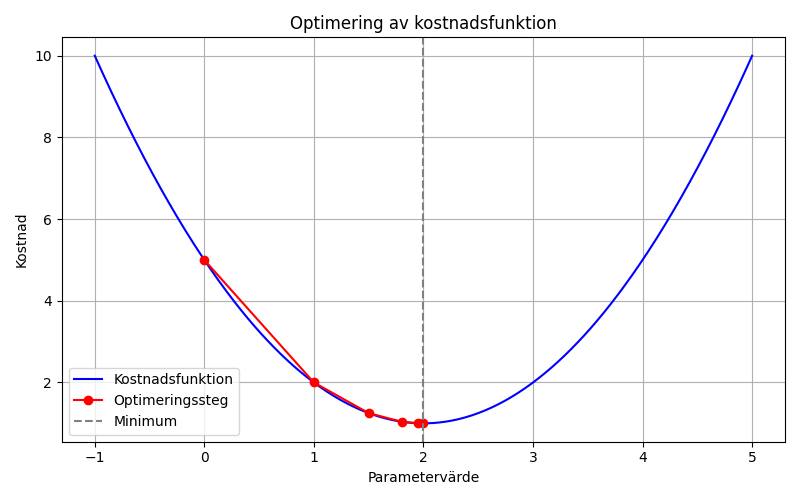
\includegraphics[width=0.55\textwidth]{optimering_kostnadsfunktion1.png}
  \end{center}
\end{frame}

\begin{frame}{Introduktion till optimering}
    \begin{figure}[htbp]
        \centering
        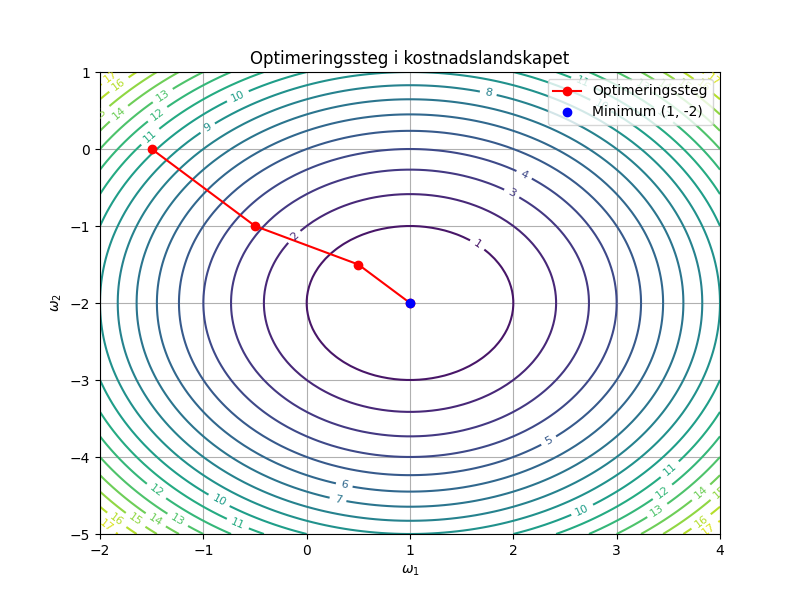
\includegraphics[width=0.6\textwidth]{optimeringssteg_konturer.png}
        \caption*{Optimeringssteg i kostnadslandskapet för 
        $f(\omega_1, \omega_2) = (\omega_1 - 1)^2 + (\omega_2 + 2)^2$}
    \end{figure}
    \begin{itemize}
        \item Konturlinjer visar nivåer av $f(\omega_1, \omega_2)$
        \item Röda punkter och linjer visar tänkta optimeringssteg
        \item Minimum vid $(1, -2)$ är markerat med blå punkt
    \end{itemize}
\end{frame}

\begin{frame}{Gradient och Euklidisk norm}
    \textbf{Gradient:}
    \begin{itemize}
        \item Gradienten av en funktion $f(x_1, x_2, \dots, x_n)$ är en vektor med partiella derivator:
        \[
        \nabla f = \left( \frac{\partial f}{\partial x_1}, \frac{\partial f}{\partial x_2}, \dots, \frac{\partial f}{\partial x_n} \right)
        \]
        \item Gradientvektorn pekar i riktningen där funktionen ökar snabbast.
        \item Kan användas i optimering för att hitta minimum eller maximum.
    \end{itemize}

    \vspace{0.4cm}
    \textbf{Euklidisk norm:}
    \begin{itemize}
        \item Normen av en vektor $v = (v_1, v_2, \dots, v_n)$ är dess längd:
        \[
        \|v\| = \sqrt{v_1^2 + v_2^2 + \dots + v_n^2}
        \]
        \item Kallas även $L^2$-norm eller den euklidiska normen.
        \item Används för att mäta storleken på gradienten.
    \end{itemize}
\end{frame}

\begin{frame}{Gradientens norm och riktining i ett kostnadslandskap}
    \begin{figure}[htbp]
        \centering
        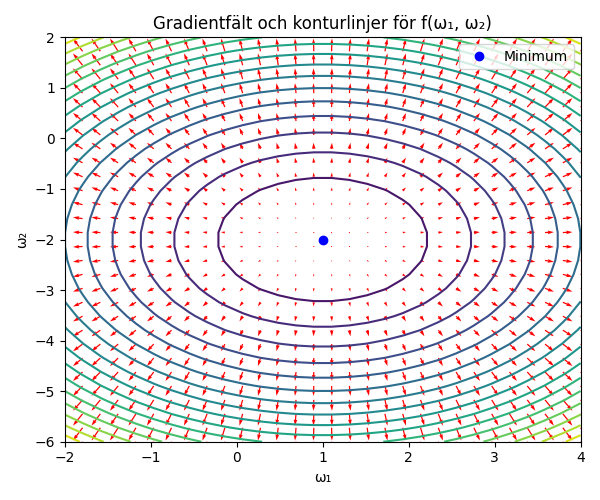
\includegraphics[width=0.5\textwidth]{gradient_landscape1.png}
        \caption*{Gradientfält och konturlinjer för $f(\omega_1, \omega_2) = 
        (\omega_1 - 1)^2 + (\omega_2 + 2)^2$}
    \end{figure}
    \begin{itemize}
        \item Konturlinjer visar nivåer av $f(\omega_1, \omega_2)$
        \item Röda pilar visar gradientens riktning och storlek
        \item Minimum vid $(1, -2)$ där gradienten är noll
    \end{itemize}
\end{frame}


\begin{frame}{Hur hittar vi de bästa värdena på $\omega$?}
    \begin{itemize}
        \item Det finns många olika sätt att lösa olika optimeringsproblem på
        \item Brute force: vi testar många värden på $\omega$ och ser vilket som ger bäst värde på $f(\omega)$ $\rightarrow$ oftast inte praktiskt genomförbart
        \item Vissa problem har enkla/analytiska lösningar
        \item Optimeringsalgoritmer som stegvis förbättrar värdet på $f(\omega)$
    \end{itemize}
\end{frame}



\begin{frame}{Minimum för en andragradsfunktion}
    Vi undersöker funktionen:
    \[
    f(x) = x^2 - 4x + 5
    \]
    \begin{itemize}
        \item Derivera funktionen:
        \[
        f'(x) = 2x - 4
        \]
        \item Sätt derivatan lika med noll:
        \[
        2x - 4 = 0 \Rightarrow x = 2
        \]
        \item Undersök andraderivatan:
        \[
        f''(x) = 2 > 0
        \]
        \item Eftersom $f''(x) > 0$ har funktionen ett \textbf{minimum} vid $x = 2$
        \item Värdet vid minimum:
        \[
        f(2) = 2^2 - 4 \cdot 2 + 5 = 4 - 8 + 5 = 1
        \]
    \end{itemize}
    \textbf{Slutsats:} Funktionen har ett minimum vid $(x, f(x)) = (2, 1)$
\end{frame}


\begin{frame}{Minimum för ett godtyckligt polynom}
    Antag att vi har ett polynom av grad $n$:
    \[
    f(x) = a_n x^n + a_{n-1} x^{n-1} + \dots + a_1 x + a_0
    \]
    \begin{itemize}
        \item \textbf{Steg 1:} Beräkna den första derivatan:
        \[
        f'(x) = n a_n x^{n-1} + (n-1) a_{n-1} x^{n-2} + \dots + a_1
        \]
        \item \textbf{Steg 2:} Sätt $f'(x) = 0$ och lös ekvationen för att hitta kritiska punkter.
        \item \textbf{Steg 3:} Beräkna den andra derivatan:
        \[
        f''(x) = n(n-1) a_n x^{n-2} + \dots
        \]
        \item \textbf{Steg 4:} Undersök tecknet på $f''(x)$ vid varje kritisk punkt:
        \begin{itemize}
            \item Om $f''(x) > 0$ $\Rightarrow$ lokalt minimum
            \item Om $f''(x) < 0$ $\Rightarrow$ lokalt maximum
            \item Om $f''(x) = 0$ $\Rightarrow$ vidare undersökning krävs
        \end{itemize}
    \end{itemize}
    \textbf{Slutsats:} Minimum hittas där $f'(x) = 0$ och $f''(x) > 0$
\end{frame}


\begin{frame}{OLS-lösning med linjär algebra}
    Vi utgår från modellen för linjär regression:
    \[
    y = X\beta + \varepsilon
    \]

    \vspace{0.3cm}
    Den klassiska OLS-lösningen för $\beta$ fås genom att minimera residualsumman:
    \[
    \min_\beta \| y - X\beta \|^2
    \]

    \vspace{0.3cm}
    Lösningen ges av:
    \[
    \hat{\beta} = (X^\top X)^{-1} X^\top y
    \]

    \begin{itemize}
        \item $X^\top X$ är en (p × p) matris
        \item $(X^\top X)^{-1}$ är inversen (om den existerar)
        \item $X^\top y$ är en (p × 1) vektor
    \end{itemize}

    \textbf{Slutsats:} Vi kan beräkna $\hat{\beta}$ direkt med linjär algebra om $X^\top X$ är inverterbar.
\end{frame}

\begin{frame}{Antaganden om värde- och definitionsmängd}
    \textbf{Antagande:}
    \begin{itemize}
        \item Kostnadsfunktionen $f(\omega)$ har de reella talen $\mathbb{R}$ som \textbf{värdemängd}.
        \item Parametern $\omega$ har de reella talen $\mathbb{R}^p$ som \textbf{definitionsmängd}.
    \end{itemize}

    \vspace{0.4cm}
    \textbf{Implikationer för optimering:}
    \begin{itemize}
        \item Vi kan använda \textbf{gradientbaserade metoder} som gradient descent.
        \item Derivator och normer är definierade och kontinuerliga.
        \item Möjligt att använda \textbf{analytiska verktyg} som första och andra derivatan.
        \item Lösningen kan ligga var som helst i det reella rummet – inga diskreta begränsningar.
    \end{itemize}

    Reell värde- och definitionsmängd möjliggör effektiv optimering med kontinuerliga metoder.
\end{frame}

\begin{frame}{Globala och lokala minimipunkter}
    \textbf{Definitioner:}
    \begin{itemize}
        \item \textbf{Lokalt minimum:} En punkt $x_0$ där $f(x_0) \leq f(x)$ för alla $x$ i en omgivning kring $x_0$.
        \item \textbf{Globalt minimum:} En punkt $x^*$ där $f(x^*) \leq f(x)$ för alla $x$ i hela definitionsmängden.
    \end{itemize}

    \vspace{0.1cm}
    \textbf{Exempel:}


    \begin{figure}[htbp]
        \centering
        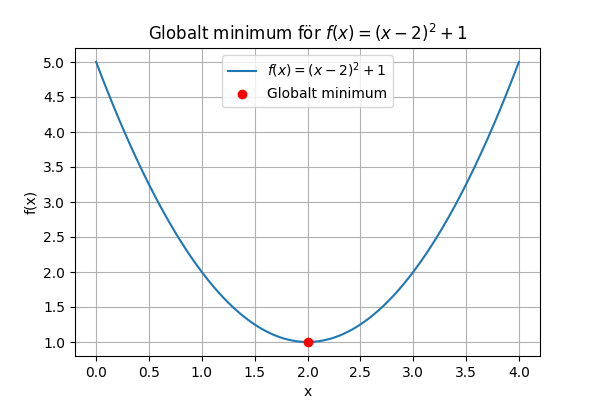
\includegraphics[width=0.45\textwidth]{globalt_min.png}
        \hspace{0.5cm}
        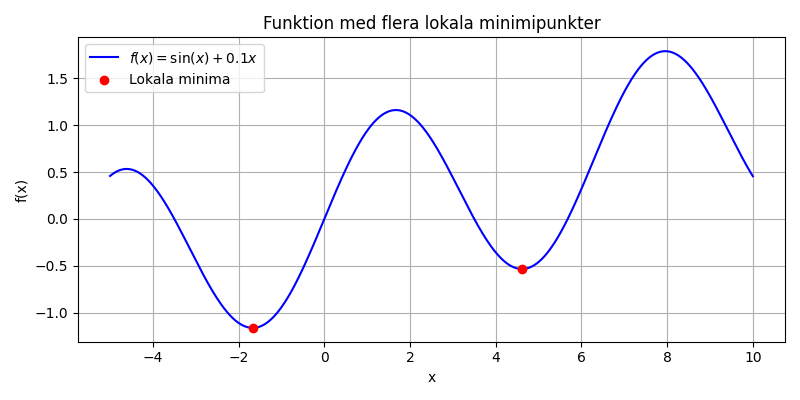
\includegraphics[width=0.45\textwidth]{lokala_minima_korrekt.png}
        \caption*{Vänster: globalt minimum. Höger: flera lokala minima.}
    \end{figure}
\end{frame}


\begin{frame}{Vad är en konvex funktion?}
    \textbf{Intuitiv förklaring:}
    \begin{itemize}
        \item En konvex funktion är "skålformad" – den böjer uppåt.
        \item Om du ritar en linje mellan två punkter på kurvan, så ligger hela linjen ovanför kurvan.
        \item Det finns bara ett minimum, och det är det lägsta värdet i hela funktionen.
    \end{itemize}

    \vspace{0.4cm}
    \textbf{Exempel:}
    \begin{itemize}
        \item $f(x) = x^2$ är en konvex funktion.
        \item $f(x) = |x|$ är också konvex – även om den har ett hörn.
    \end{itemize}

    \vspace{0.4cm}
    \textbf{Varför är det bra?}
    \begin{itemize}
        \item Enklare att hitta minimum – vi vet att det inte finns några "fällor".
        \item Optimeringsalgoritmer fungerar bättre och snabbare.
    \end{itemize}
\end{frame}

\begin{frame}{Konvexa och icke-konvexa funktioner}

    \textbf{Icke-konvex funktion:}
    \begin{itemize}
        \item Bryter mot konvexitetsvillkoret.
        \item Kan ha \textbf{flera lokala minima} och maxima.
        \item Exempel: $f(x) = \sin(x)$, $f(x) = x^4 - x^2$
    \end{itemize}

    \vspace{0.3cm}
    \textbf{Konsekvenser för optimering:}
    \begin{itemize}
        \item Konvexa funktioner: enklare att optimera, globalt minimum kan hittas med gradientmetoder.
        \item Icke-konvexa funktioner: kräver mer avancerade metoder (t.ex. randomisering, flera startpunkter). Vi har inga garantier att hitta ett globalt minimium.
    \end{itemize}
\end{frame}


\begin{frame}{En generisk optimeringsalgoritm}
  \begin{itemize}
    \item Starta med en initial parametervektor \( \omega_0 \)
    \item Sätt ett max antal iterationer \( k \)
  \end{itemize}

  \vspace{1em}
  \textbf{För varje iteration } \( i = 1, 2, \dots, k \):
  \begin{enumerate}
    \item Uppdatera \( \omega_i \) baserat på \( \omega_{i-1} \) enligt en specifik regel
    \item Beräkna kostnaden \( f\left(\omega_i\right) \)
    \item Undersök konvergens:
    \begin{itemize}
      \item Om konvergerat: avbryt loopen
    \end{itemize}
  \end{enumerate}

  \vspace{0.5em}
  \textbf{Returnera:} \( \omega_i \) och \( f\left(\omega_i\right) \)
\end{frame}


\begin{frame}{Vad menas med konvergens?}
  \begin{itemize}
    \item En optimeringsalgoritm sägs ha \textbf{konvergerat} när den når ett tillstånd där ytterligare iterationer inte leder till någon meningsfull förbättring.
    \item Det finns flera sätt att definiera konvergens:
    \begin{itemize}
      \item \textbf{Liten förändring i kostnadsfunktionen:} \\
        \( |f(\omega_{i}) - f(\omega_{i-1})| < \varepsilon_{1} \)
      \item \textbf{Liten förändring i parametrarna:} \\
        \( \|\omega_{i} - \omega_{i-1}\| < \varepsilon_{2} \)
      \item \textbf{Gradientens norm är nära noll:} \\
        \( \|\nabla f(\omega_{i})\| < \varepsilon_{3} \)
      \item \textbf{Maximalt antal iterationer har uppnåtts}
    \end{itemize}
    \item Valet av konvergenskriterium påverkar både hur bra den föreslagna lösningen blir och beräkningstiden.
  \end{itemize}
\end{frame}

\begin{frame}{Gradient Descent – En optimeringsmetod}
    \textbf{Vad är Gradient Descent?}
    \begin{itemize}
        \item En metod för att hitta minimum av en funktion.
        \item Används ofta för att minimera kostnadsfunktioner i maskininlärning.
        \item Bygger på att följa den negativa riktningen av gradienten.
    \end{itemize}

    \textbf{Hur fungerar det?}
    \begin{itemize}
        \item Starta från en initial punkt $\omega_0$.
        \item Uppdatera enligt: 
        \[
        \omega_{t+1} = \omega_t - \gamma \nabla f(\omega_t)
        \]
        där $\gamma$ är inlärningshastigheten (stegets storlek).
        \item Upprepa tills gradienten är nära noll (dvs. vi når ett minimum).
    \end{itemize}

    \textbf{Nyckelidéer:}
    \begin{itemize}
        \item Gradient = riktning där funktionen ökar mest.
        \item Negativ gradient = riktning mot lägre värden.
        \item Inlärningshastigheten påverkar hur snabbt vi rör oss mot bättre värden.
    \end{itemize}
\end{frame}

\begin{frame}{Gradient Descent – Visuell illustration}
    \begin{figure}[htbp]
        \centering
        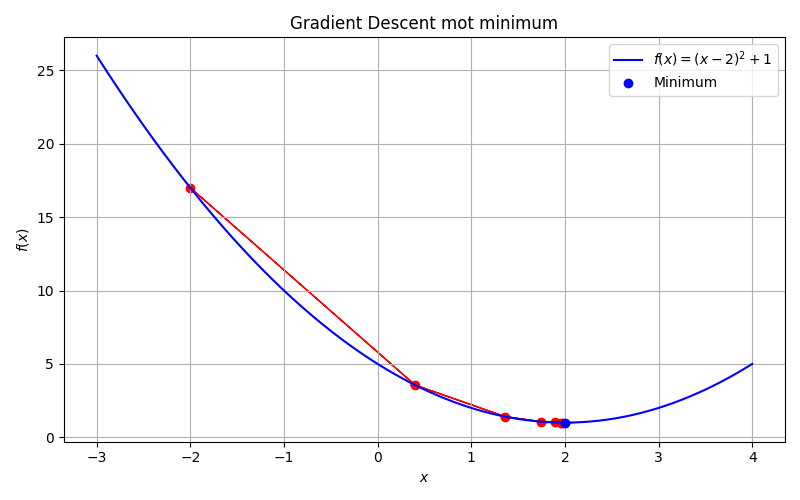
\includegraphics[width=0.7\textwidth]{gradient_descent_figur.png}
        \caption*{Gradient descent mot minimum för $f(x) = (x - 2)^2 + 1$}
    \end{figure}

    \begin{itemize}
        \item Startpunkt vid $x=-2$
        \item Pilar visar hur algoritmen rör sig mot lägre värden
        \item Stegen följer den negativa gradienten
        \item Minimum nås vid $x = 2$
    \end{itemize}
\end{frame}

\begin{frame}{Gradient Descent i flera dimensioner – 3D-visualisering}
    \begin{figure}[htbp]
        \centering
        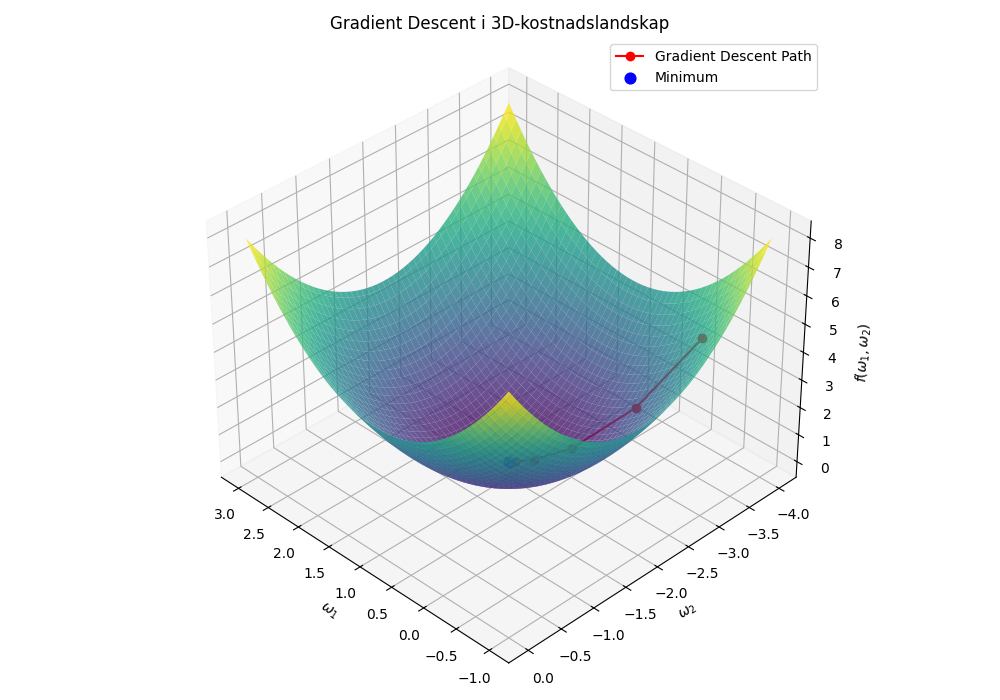
\includegraphics[width=0.77\textwidth]{gradient_descent_3d_rotated.png}
        \caption*{Gradient descent i ett 3D-kostnadslandskap: $f(\omega_1, \omega_2) = (\omega_1 - 1)^2 + (\omega_2 + 2)^2$}
    \end{figure}

    \begin{itemize}
        \item Ytan visar kostnadsfunktionen som beror på två variabler.
        \item Den röda linjen visar optimeringsstegen från startpunkt till minimum.
    \end{itemize}
\end{frame}

\begin{frame}{När konvergerar Gradient Descent?}
    \textbf{För att Gradient Descent ska konvergera till ett lokalt minimum krävs:}
    \begin{itemize}
        \item \textbf{Funktionen $f(\omega)$ är differentiabel:} Vi måste kunna beräkna gradienten.
        \item \textbf{Gradienten är Lipschitz-kontinuerlig:} Det finns en konstant $L$ så att
        \[
        \|\nabla f(\omega_1) - \nabla f(\omega_2)\| \leq L \|\omega_1 - \omega_2\|
        \]
        vilket ger stabilitet i uppdateringarna.
        \item \textbf{Inlärningshastigheten $\gamma$ är tillräckligt liten:} Om $\gamma < \frac{2}{L}$ så garanteras konvergens.
        \item \textbf{Startpunkt nära minimum:} För icke-konvexa funktioner kan algoritmen fastna i lokala minima.
        \item \textbf{Funktionen är konvex (för global konvergens):} Då är varje lokalt minimum också ett globalt minimum.
    \end{itemize}

    Med rätt förutsättningar leder gradient descent till ett (lokalt) minimum.
\end{frame}

\begin{frame}{Gradient Descent – Steglängdens roll}
  \begin{itemize}
    \item Vi optimerar funktionen $f(x) = x^2$ med gradient descent.
    \item Startpunkt: $x = 8$, antal iterationer: 20.
    \item \textbf{För liten steglängd (0.05):} långsam konvergens.
    \item \textbf{Lagom steglängd (0.2):} snabb och stabil konvergens.
    \item \textbf{För stor steglängd (0.8):} hoppar över minimum, risk för divergens.
  \end{itemize}
  \begin{center}
    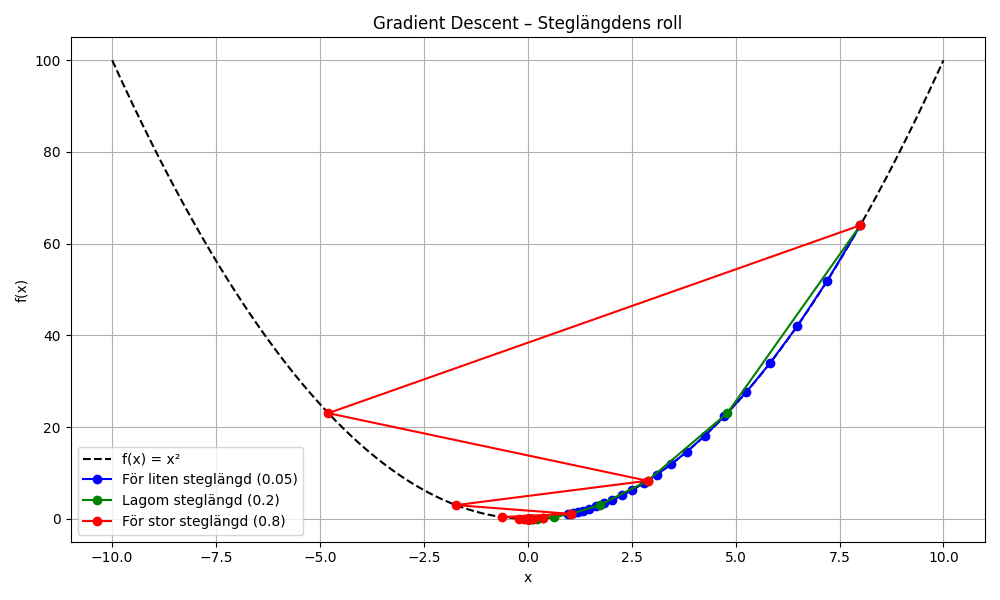
\includegraphics[width=0.87\textwidth]{steglangd_gradient_descent.png}
  \end{center}
\end{frame}

\begin{frame}{Gradient Descent: Fördelar och nackdelar}
  \begin{columns}
    \column{0.48\textwidth}
    \textbf{Fördelar}
    \begin{itemize}
      \item Enkel att implementera
      \item Fungerar för stora datamängder
      \item Flexibel för olika typer av modeller
      \item Kan användas med olika förbättringar/utökningar
    \end{itemize}

    \column{0.48\textwidth}
    \textbf{Nackdelar}
    \begin{itemize}
      \item Känslig för val av steglängd
      \item Kan fastna i lokala minima
      \item Långsam konvergens
      \item Kräver derivator av målfunktionen
    \end{itemize}
  \end{columns}
\end{frame}

\begin{frame}{Vanliga förbättringar av Gradient Descent}
  \begin{itemize}
    \item Stochastic Gradient Descent (SGD)
    \item Momentum
    \item Nesterov Accelerated Gradient
    \item Adagrad
    \item RMSprop
    \item Adam
    \item AdaDelta
    \item Learning rate scheduling/Steglängdsscheman
  \end{itemize}
\end{frame}

\begin{frame}{Gradient Descent – Steglängdsscheman}
  \begin{itemize}
    \item Ett \textbf{steglängdsschema} är en metod för att ändra steglängden $\gamma$ över iterationer i gradient descent.
    \item Syftet är att börja med en större steglängd för snabb konvergens, och sedan minska den för stabilitet.
    \item Vanligt schema: $\gamma_t = \frac{\gamma_0}{1 + \alpha t}$ där $\gamma_0$ är initial steglängd och $\alpha$ styr minskningstakten.
    \item Hjälper algoritmen att undvika att studsa runt minimum i senare iterationer.
  \end{itemize}
  \begin{center}
    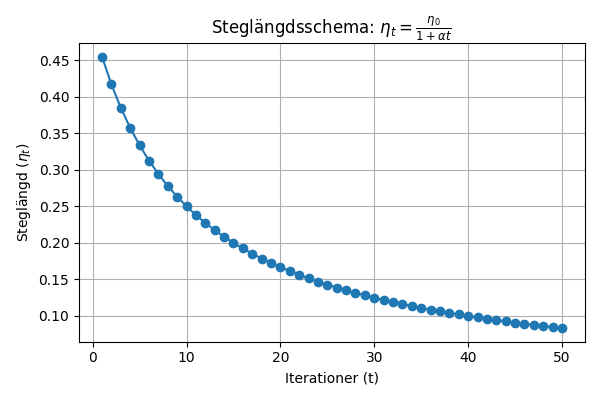
\includegraphics[width=0.55\textwidth]{steglangdsschema.png}
  \end{center}
\end{frame}


\begin{frame}{Gradient Descent för Multipel Linjär Regression}
  \begin{itemize}
    \item Vi modellerar sambandet mellan flera variabler med:
    \[
      \mathbf{y} = \mathbf{X} \boldsymbol{\beta}
    \]
    där:
    \begin{itemize}
      \item $\mathbf{y}$ är en $n \times 1$-vektor med utfall,
      \item $\mathbf{X}$ är en $n \times p$-matris med prediktorer (inkl. intercept),
      \item $\boldsymbol{\beta}$ är en $p \times 1$-vektor med koefficienter.
    \end{itemize}
    \item Kostnadsfunktion (MSE):
    \[
      f(\boldsymbol{\beta}) = \frac{1}{n} (\mathbf{y} - \mathbf{X}\boldsymbol{\beta})^\top (\mathbf{y} - \mathbf{X}\boldsymbol{\beta})
    \]
    \item Gradienten ges av:
    \[
      \nabla f(\boldsymbol{\beta}) = -\frac{2}{n} \mathbf{X}^\top (\mathbf{y} - \mathbf{X}\boldsymbol{\beta})
    \]
    \item Uppdateringsregel:
    \[
      \boldsymbol{\beta} := \boldsymbol{\beta} - \gamma \cdot \nabla f(\boldsymbol{\beta})
    \]
    där $\gamma$ är steglängden.
  \end{itemize}
\end{frame}

\begin{frame}{Coordinate Descent – En variabel i taget}
    \textbf{Vad är Coordinate Descent?}
    \begin{itemize}
        \item En optimeringsmetod där man optimerar en variabel i taget.
        \item Alla andra variabler hålls fasta under varje steg.
        \item Itererar över variablerna tills konvergens uppnås.
    \end{itemize}

    \vspace{0.3cm}
    \textbf{Nyckelidéer:}
    \begin{itemize}
        \item Enkel att implementera, särskilt för stora problem.
        \item Effektiv när varje delproblem (en variabel) är lätt att lösa.
        \item Används ofta i t.ex. Lasso-regression (mer om det senare) och konvex optimering.
        \item Kräver inte beräkning av hela gradienten.
    \end{itemize}
\end{frame}

\begin{frame}{Första och andra ordningens metoder}
  \begin{itemize}
    \item \textbf{Första ordningens metoder:}
    \begin{itemize}
      \item Använder endast gradienten (första derivatan) av kostandsfunktionen.
      \item Exempel: Gradient Descent, Stochastic Gradient Descent.
    \end{itemize}
    \item \textbf{Andra ordningens metoder:}
    \begin{itemize}
      \item Använder både gradienten och Hessianen (andra derivatan).
      \item Exempel: Newtons metod, Quasi-Newton (t.ex. BFGS).
    \end{itemize}
    \item Val mellan metoder beror på problemets struktur, resurser och krav på noggrannhet.
  \end{itemize}
\end{frame}

\begin{frame}{Vad är en Hessian?}
  \begin{itemize}
    \item Hessianen är en matris med alla andra ordningens partialderivator av en funktion.
    \item Används i optimering för att analysera kurvatur och hitta extrema punkter.
    \item \textbf{Exempel:} Funktionen \( f(x, y) = x^2 + xy + y^2 \)
  \end{itemize}
  \[
  \nabla^2 f(x, y) =
  \begin{bmatrix}
    \frac{\partial^2 f}{\partial x^2} & \frac{\partial^2 f}{\partial x \partial y} \\
    \frac{\partial^2 f}{\partial y \partial x} & \frac{\partial^2 f}{\partial y^2}
  \end{bmatrix}
  =
  \begin{bmatrix}
    2 & 1 \\
    1 & 2
  \end{bmatrix}
  \]
\end{frame}

\begin{frame}{Exempel på Hessian: Funktion med tre variabler}
  \begin{itemize}
    \item Funktion: \( f(x, y, z) = x^2 + xy + y^2z + \sin(z) \)
    \item Hessianen innehåller alla andra ordningens partialderivator:
  \end{itemize}
  \[
  \nabla^2 f(x, y, z) =
  \begin{bmatrix}
    \frac{\partial^2 f}{\partial x^2} & \frac{\partial^2 f}{\partial x \partial y} & \frac{\partial^2 f}{\partial x \partial z} \\
    \frac{\partial^2 f}{\partial y \partial x} & \frac{\partial^2 f}{\partial y^2} & \frac{\partial^2 f}{\partial y \partial z} \\
    \frac{\partial^2 f}{\partial z \partial x} & \frac{\partial^2 f}{\partial z \partial y} & \frac{\partial^2 f}{\partial z^2}
  \end{bmatrix}
  =
  \begin{bmatrix}
    2 & 1 & 0 \\
    1 & 2z & y^2 \\
    0 & y^2 & -\sin(z)
  \end{bmatrix}
  \]
\end{frame}

\begin{frame}{Viktiga andra ordningens optimeringsmetoder}
  \begin{itemize}
    \item Newtons metod
    \item Quasi-Newton-metoder
    \begin{itemize}
      \item BFGS (Broyden–Fletcher–Goldfarb–Shanno)
      \item L-BFGS (Limited-memory BFGS)
      \item DFP (Davidon–Fletcher–Powell)
    \end{itemize}
    \item Gauss-Newton-metoden
    \item Conjugate Gradient (för icke-linjär optimering)
  \end{itemize}
\end{frame}

\begin{frame}{Begränsningar via reparameterisering}
  \begin{itemize}
    \item Ibland måste parametrar uppfylla vissa villkor, t.ex. vara positiva.
    \item Istället för att optimera direkt på parametern, kan vi omformulera problemet.
    \item \textbf{Exempel:} Om \( \theta > 0 \), optimera istället över \( \phi \) där:
    \[
    \theta = \exp(\phi)
    \]
    \item Nu är \( \theta \) alltid positiv, oavsett värde på \( \phi \).
    \item Reparameterisering gör det möjligt att använda gradientbaserade metoder utan att hantera begränsningar direkt.
  \end{itemize}
\end{frame}

\begin{frame}{Värdemängd och definitionsmängd i optimering}
    \textbf{Värdemängd för $f(\omega)$:}
    \begin{itemize}
        \item Värdemängden är alla möjliga utfall av kostnadsfunktionen $f(\omega)$.
        \item Exempel: Om $f(\omega) = \|\omega\|^2$ är värdemängden $[0, \infty)$.
    \end{itemize}

    \vspace{0.2cm}
    \textbf{Definitionsmängd för $\omega$:}
    \begin{itemize}
        \item \textbf{Reella tal:} $\omega \in \mathbb{R}^p$ $\Rightarrow$ gradientbaserade metoder som gradient descent kan användas.
        \item \textbf{Heltal:} $\omega \in \mathbb{Z}^p$ $\Rightarrow$ diskreta metoder som branch-and-bound eller dynamisk programmering krävs.
        \item \textbf{Intervall:} $\omega \in [a, b]^p$ $\Rightarrow$ optimering med begränsningar, t.ex. projicerad gradient descent eller L-BFGS-B.
        \item \textbf{Blandade variabler:} Kombination av reella och heltal $\Rightarrow$ mixed-integer programming (MIP).
    \end{itemize}

    Valet av optimeringsalgoritm beror på både värdemängden för $f(\omega)$ och definitionsmängden för $\omega$.
\end{frame}

\begin{frame}{Optimering i modellering}
  \begin{itemize}
    \item Optimering är centralt för att träna/skatta modeller inom statistik och maskininlärning.
    \item Målet är ofta att minimera en förlustfunktion eller maximera en sannolikhet.
    \item \textbf{Exempel:}
    \begin{itemize}
      \item Linjär regression: minimera residualsumma
      \item Logistisk regression: maximera log-likelihood
      \item Regulariserade modeller: balansera förlust och komplexitet
      \item Neurala nätverk: minimera förlust via gradientbaserade metoder
    \end{itemize}
    \item Val av optimeringsmetod påverkar både noggrannhet och effektivitet.
  \end{itemize}
\end{frame}


\begin{frame}{Parametrar vs. Hyperparametrar}
  \begin{itemize}
    \item \textbf{Parametrar:}
    \begin{itemize}
      \item Lärs direkt från data under träning.
      \item Exempel: parametrar i en linjär (logistisk) regressionsmodell
    \end{itemize}
    \item \textbf{Hyperparametrar:}
    \begin{itemize}
      \item Ställs in före träning av parametarna
      \item "Styr modellens/skattningens övergripande egenskaper"
      \item Kan handla dels om modellen, men också om hur vi skattar modellens parametrar
      \item Skattning/optimiering, exempel: val av algoritm, lärhastighet, antal iterationer, regulariseringsstyrka
      \item Modellens struktur kan vara en hyperparameter:
      \begin{itemize}
        \item Antal variabler eller features
        \item Val av modelltyp (t.ex. linjär vs. icke-linjär)
        \item Antal lager i ett neuralt nätverk
      \end{itemize}
    \end{itemize}
    \item Vi kan inte skatta hyperparametrar på "vanligt" sätt $\rightarrow$ leder ofta till överanpassning
  \end{itemize}
\end{frame}

\begin{frame}{Val av hyperparametrar med validering}
  \begin{itemize}
    \item Hyperparametrar styr modellens träning och struktur.
    \item För att välja bra värden testar vi olika alternativ och utvärderar modellen.
    \item \textbf{Validering:}
    \begin{itemize}
      \item Dela upp data i tränings- och valideringsdel.
      \item Träna modellen på träningsdata, utvärdera på valideringsdata.
    \end{itemize}
    \item \textbf{Korsvalidering:}
    \begin{itemize}
      \item Dela upp data i flera delar (folds).
      \item Träna och utvärdera modellen flera gånger med olika uppdelningar.
      \item Vanligt: 5- eller 10-faldig korsvalidering.
    \end{itemize}
    \item Välj de hyperparametrar som ger bäst genomsnittlig prestanda.
    \item Vilka värden ska vi välja? Grid search, random search, ...
  \end{itemize}
\end{frame}

\begin{frame}{Frågor?}
    
\end{frame}

\end{document}